% ---------------------------------------------------------------------------
% Threshold-selection evidence for the GPU predictive watchdog (paste into the
% watchdog / L7 section). Figure: figures/fig_throttle_threshold.{png,pdf}
% Framing: we do NOT claim discovery of skin/battery-governed throttling. The
% MECHANISM (Thermal Engine: config-file frequency caps, PID on temperature
% sensors incl. skin) is documented by Bantock et al. [bantock2020thermal];
% the onset TEMPERATURES are OEM-configured per device, so we measure OURS
% (clustering over 27 traces) and cite the figure as threshold justification.
% ---------------------------------------------------------------------------
\begin{figure}[t]
  \centering
  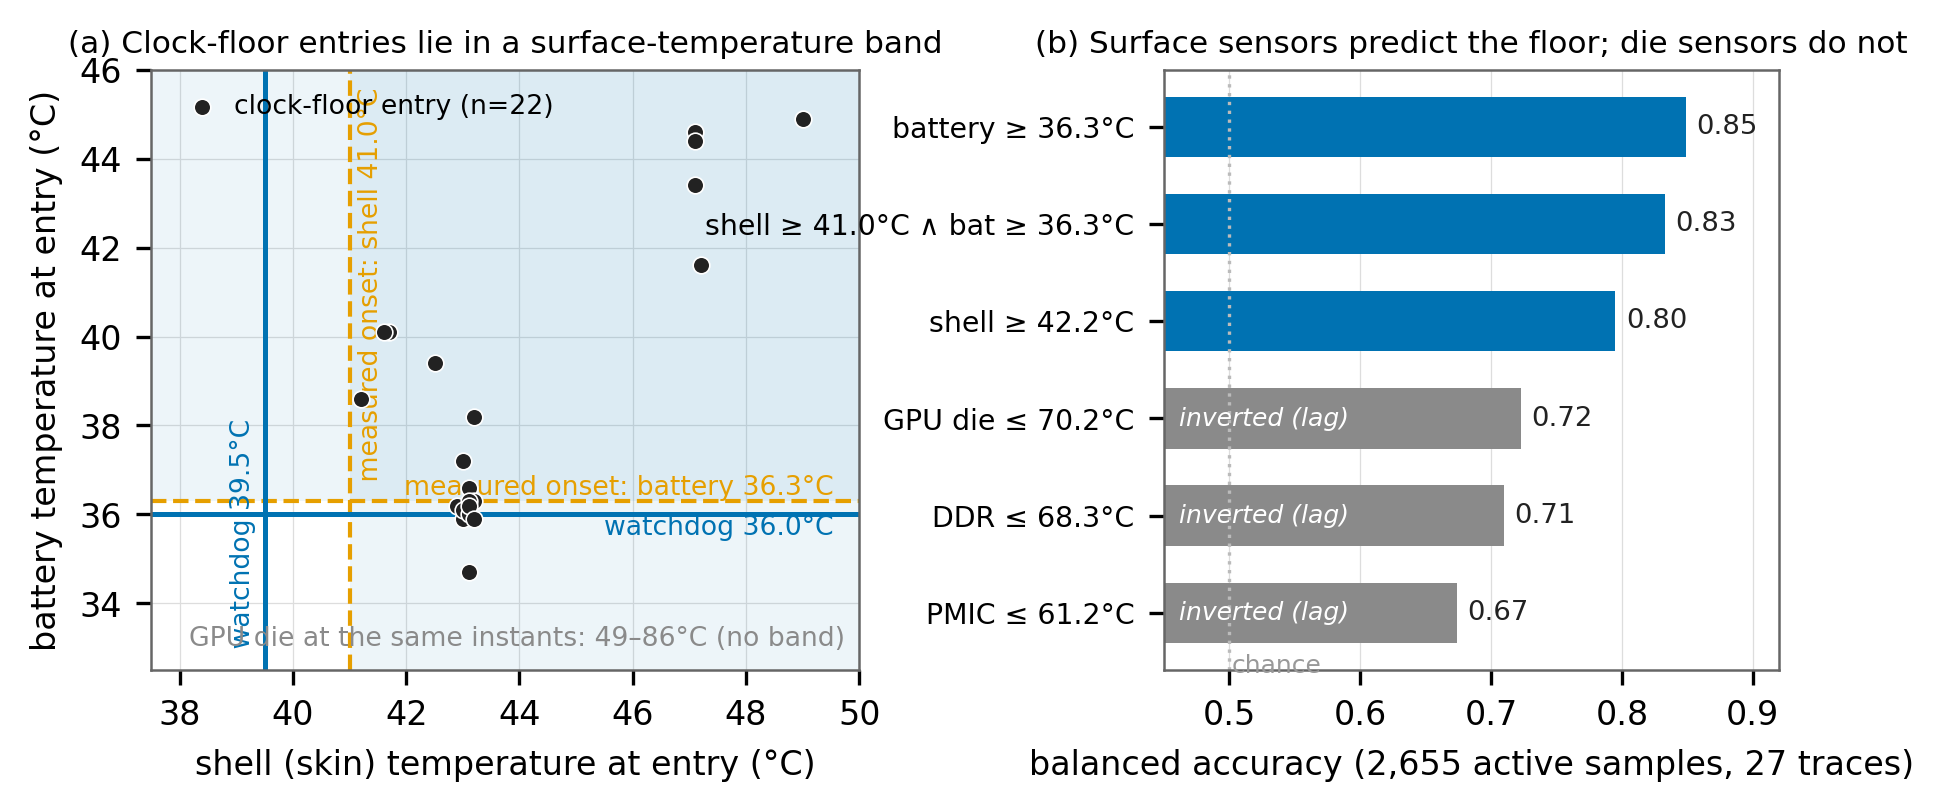
\includegraphics[width=\linewidth]{figures/fig_throttle_threshold.png}
  \caption{\textbf{Evidence-based watchdog thresholds.} \emph{(a)} All 22
  sustained GPU clock-floor entries found across 27 dynamic-clock traces
  (2{,}655 active samples) on the OnePlus~15 lie in a narrow
  \emph{surface}-temperature band (shell $\geq$41\,\textdegree C; battery
  clustered at 36--37\,\textdegree C), while GPU-die temperature at the same
  instants spans 49--86\,\textdegree C --- the die sensors carry no onset
  band. This is consistent with the documented mechanism: Qualcomm's Thermal
  Engine applies configuration-file frequency caps, driven by a PID controller
  over temperature sensors including \emph{skin} temperature, with onset
  values configured per device by the OEM~\cite{bantock2020thermal}; the
  $\sim$30\,s lag between die heating and the cap explains why die sensors
  are already \emph{cooling} when the floor engages. \emph{(b)} Separator
  quality over the same samples: battery ($\geq$36.3\,\textdegree C, balanced
  accuracy 0.85) and shell ($\geq$42.2\,\textdegree C, 0.80) predict the
  floor; die sensors (GPU/DDR/PMIC) only separate through \emph{inverted}
  rules --- the lag artifact --- and are unusable as a forward guard. The
  watchdog therefore triggers on shell$\,\geq$39.5\,\textdegree C $\wedge$
  battery$\,\geq$36.0\,\textdegree C, one step \emph{before} the measured
  onset, and steps the clock down the \emph{vendor-authorized} frequency
  table (read from \texttt{/sys/kernel/gpu/gpu\_freq\_table}: 1200, 1050,
  967, 902, 826\,MHz), holding an intermediate authorized rung instead of
  letting the Thermal Engine collapse the clock deep into its 18-level
  ladder.}
  \label{fig:throttle-threshold}
\end{figure}

% Verified citation (mechanism only; onset temps are OEM-configured, ours are
% measured). IEEE Xplore 9081929; ePrints Soton 439709.
%
% @article{bantock2020thermal,
%   title   = {Mitigating Interactive Performance Degradation From Mobile
%              Device Thermal Throttling},
%   author  = {Bantock, James and Bright, Robert Benjamin and
%              Al-Hashimi, Bashir M. and Merrett, Geoff V.},
%   journal = {IEEE Transactions},
%   year    = {2020},
%   note    = {Qualcomm Thermal Engine: configuration-file frequency caps,
%              PID controller over temperature sensor readings; skin-driven
%              throttling. Verify exact venue/volume from IEEE Xplore
%              document 9081929 before camera-ready.}
% }
